\section{Results}
\label{sec:results}

%\textit{Analysis: of results and the effectiveness of their selection and presentation. Are the results well understood and discussed?}

In this section I am presenting the main results of the current project. I have to run code both for generating artificial data set as described in previous sections, as well as on the real one.

\subsection{Generated/"Fake" data set}
\subsubsection{OLS, Ridge and Lasso regressions on Franke Function}
For artificial data set, I have used polynomial up to 8th degree with the generated grids of $10\times10$, $21\times21$, $50\times50$ and $100\times100$ points and hyper parameter, $\lambda$, ranging from $0.0001$ to $0.1$. Please note, that such value for the polynomial is not the limited one - the only limitation is the amount of memory on your machine. The results of the runs, for \textit{MSE}s and $R^2$  for two "extreme" cases - $10\times10$ and $100\times100$ are summarized in the tables \ref{table:all-mse1}-\ref{table:all-mse2}. \textbf{Note}: I didn't save these values inside "txt" files, instead they appear directly as a print statements in the console.

\begin{table}[h!]
\begin{tabular}{ |p{2cm}|p{3cm}|p{3cm}|p{3cm}|p{3cm}|  }
 \hline
 \multicolumn{5}{|c|}{Regression Type} \\
 \hline
 Polynomial \newline Degree & Linear \newline MSE, $R^2$ & Ridge \newline MSE, $R^2$ & Lasso \newline MSE, $R^2$  & Type\\
 \hline
 1 & 0.0304, 0.659 \newline 0.0304, 0.659 &0.0304, 0.659 \newline 0.0304, 0.659 &   0.0304, 0.659 & Scikit Learn \newline Manual\\
 \hline
 2 & 0.0259, 0.709 \newline 0.0259, 0.709  & 0.0259, 0.709 \newline 0.0259, 0.709   & 0.0259, 0.709 & Scikit Learn \newline Manual\\
 \hline
 3 & 0.0153, 0.828 \newline 0.0153, 0.828 & 0.0153, 0.828 \newline 0.0153, 0.828 &  0.0153, 0.828 & Scikit Learn \newline Manual\\
 \hline
 4 & 0.0153, 0.828 \newline .0153, 0.828 & 0.0153, 0.828 \newline 0.0153, 0.828 &  0.0159, 0.821 & Scikit Learn \newline Manual\\
 \hline
 5 & 0.0132, 0.851 \newline 0.0132, 0.851 & 0.0134, 0.849 \newline 0.0134, 0.849 & 0.0156, 0.824 & Scikit Learn \newline Manual\\
 \hline
 6 & 0.0103, 0.884 \newline 0.0103, 0.884 & 0.0118, 0.8676 \newline 0.0118, 0.8676  & 0.01091, 0.877 & Scikit Learn \newline Manual\\
 \hline
 7 & 0.0075, 0.9158 \newline 0.00998, 0.888 & 0.01060, 0.8813 \newline 0.01060, 0.8786 & 0.01740, 0.8126 & Scikit Learn \newline Manual\\
 \hline
 8 & 0.01022, 0.8899 \newline 0.01022, 0.8899 & 0.01118, 0.87967 \newline 0.01118, 0.87967 & 0.01678, 0.81944 & Scikit Learn \newline Manual\\
 \hline
\end{tabular}
\caption{Comparison of results for the fitting of several different regression models to the generated data set. Grid is $10\times10$ points and $\lambda = 0.0001$.}
\label{table:all-mse1}
\end{table}

\begin{table}[h!]
\begin{tabular}{ |p{2cm}|p{3cm}|p{3cm}|p{3cm}|p{3cm}|  }
 \hline
 \multicolumn{5}{|c|}{Regression Type} \\
 \hline
 Polynomial \newline Degree & Linear \newline MSE, $R^2$ & Ridge \newline MSE, $R^2$ & Lasso \newline MSE, $R^2$  & Type\\
 \hline
 1 & 0.0336, 0.637 \newline 0.0336, 0.637 & 0.0336, 0.637 \newline 0.0336, 0.637 &   0.0336, 0.637 & Scikit Learn \newline Manual\\
 \hline
 2 & 0.0271, 0.707 \newline 0.0271, 0.707  & 0.0271, 0.707 \newline 0.0271, 0.707   & 0.0271, 0.707 & Scikit Learn \newline Manual\\
 \hline
 3 & 0.018, 0.805 \newline 0.018, 0.805 & 0.018, 0.805 \newline 0.018, 0.805 &  0.0186, 0.799 & Scikit Learn \newline Manual\\
 \hline
 4 & 0.0142, 0.846 \newline 0.0142, 0.846 & 0.0142, 0.846 \newline 0.0142, 0.846 &  0.0188, 0.7975 & Scikit Learn \newline Manual\\
 \hline
 5 & 0.0122, 0.868 \newline 0.0122, 0.868 & 0.0122, 0.868 \newline 0.0122, 0.868 & 0.019, 0.7952 & Scikit Learn \newline Manual\\
 \hline
 6 & 0.0111, 0.8800 \newline 0.0111, 0.8800 & 0.01159, 0.8752 \newline 0.01159, 0.8752 & 0.01817, 0.8044 & Scikit Learn \newline Manual\\
 \hline
 7 & 0.01050, 0.8870 \newline 0.01050, 0.8870 & 0.01127, 0.8813 \newline 0.01127, 0.8786 & 0.01740, 0.8126 & Scikit Learn \newline Manual\\
 \hline
 8 & 0.01119, 0.894 \newline 0.01120, 0.8894 & 0.01125, 0.893 \newline 0.0154, 0.87967 & 0.0154, 0.8266 & Scikit Learn \newline Manual\\
 \hline
\end{tabular}
\caption{Comparison of results for the fitting of several different regression models to the generated data set. Grid is $100\times100$ points and $\lambda = 0.0001$.}
\label{table:all-mse2}
\end{table}

 The first set of values obtained through manual algorithm implementation, while the second row is the comparison to the Scikit Learn. As I've already mentioned before, I have not implemented manual algorithm for Lasso regression, but instead was using only scikit learn functionalities. As we can see, they are almost identical, with the Lasso algorithm being slightly behind. The value $\lambda=0.0001$ is empirical.
 
 Such high values of $R^2$ squared (and low MSE values) are generally a good thing. However, the danger here is that it can be also the sign of the model overfitting. Indeed, in figures \rf{fig:linear-surf1}-\rf{fig:lasso-surf2}, you can see the corresponding surfaces of real data, predicted values via manual algorithm and also Scikit Learn analog. The top row shows underfitting, instead of a complex surface, we have a straight one. It improves later on, the more complex our model becomes. However, at some point the model starts overfit the data. This feature is quite evident on both data sets, i.e. on the bottom plot - on the endges our models started to fit noise.
 
 %%%%%%%%%%%%%%%%%%%%%%%%%%%%%%%%%%%%%%%%%%%%%%%%%%%%%%%%%%%%%%%%%%%%%%%%%%%%%%%%%%%%%
 % Surfaces
 %%%%%%%%%%%%%%%%%%%%%%%%%%%%%%%%%%%%%%%%%%%%%%%%%%%%%%%%%%%%%%%%%%%%%%%%%%%%%%%%%%%%%
\begin{figure}[!ht]
\begin{subfigure}{\textwidth}
  \centering
  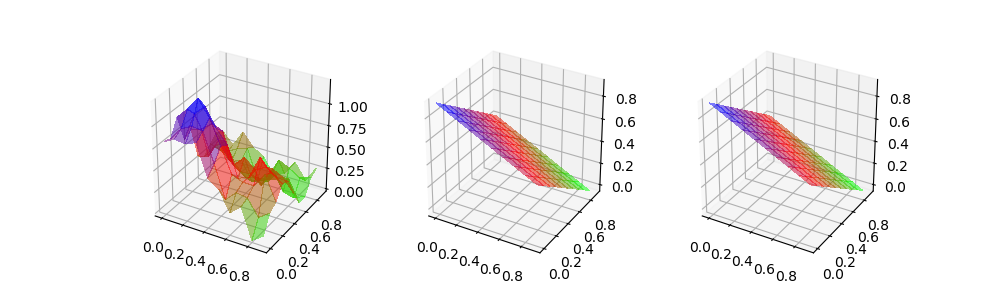
\includegraphics[width=1\linewidth]{images/surf/fake_linear_p01_n10.png}
  %\caption{}
  %\label{fig:v_x}
\end{subfigure}
\begin{subfigure}{\textwidth}
  \centering
  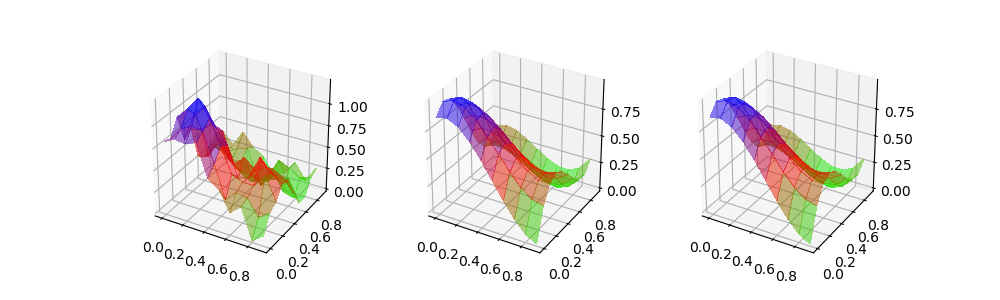
\includegraphics[width=1\linewidth]{images/surf/fake_linear_p03_n10.png}
  %\caption{}
  %\label{fig:vb_x}
\end{subfigure}
\begin{subfigure}{\textwidth}
  \centering
  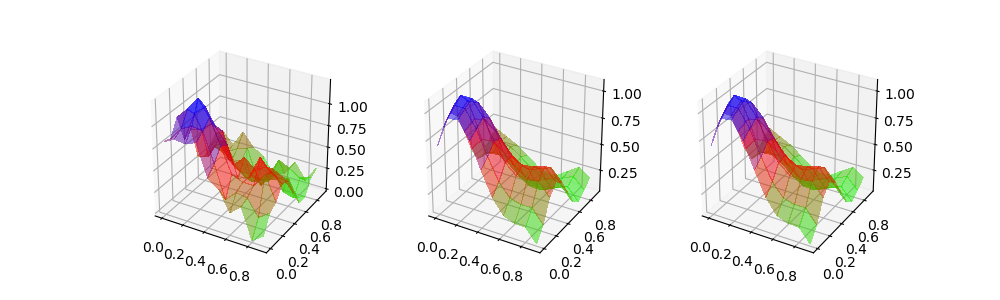
\includegraphics[width=1\linewidth]{images/surf/fake_linear_p05_n10.png}
  %\caption{}
  %\label{fig:v_x}
\end{subfigure}
\begin{subfigure}{\textwidth}
  \centering
  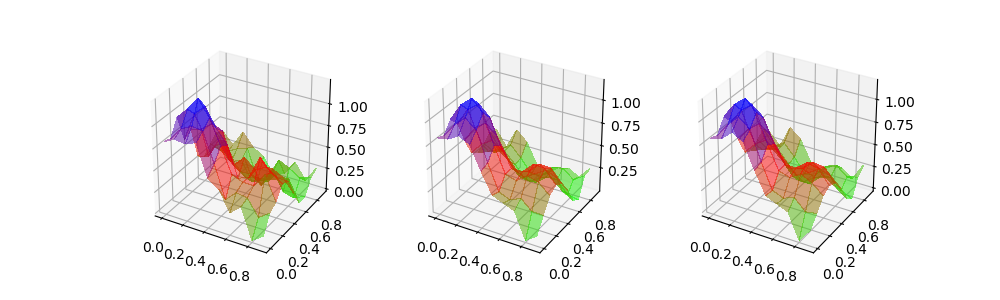
\includegraphics[width=1\linewidth]{images/surf/fake_linear_p08_n10.png}
  %\caption{}
  %\label{fig:v_x}
\end{subfigure}
\caption{The 3D visualisation of the noisy data set (left column) and the predicted surface via Lasso regression (right column) for polynomials 1, 3, 5 and 8 (from top to bottom). Grid is $10\times10$ points.}
\label{fig:linear-surf1}
\end{figure}

\begin{figure}[!ht]
\begin{subfigure}{\textwidth}
  \centering
  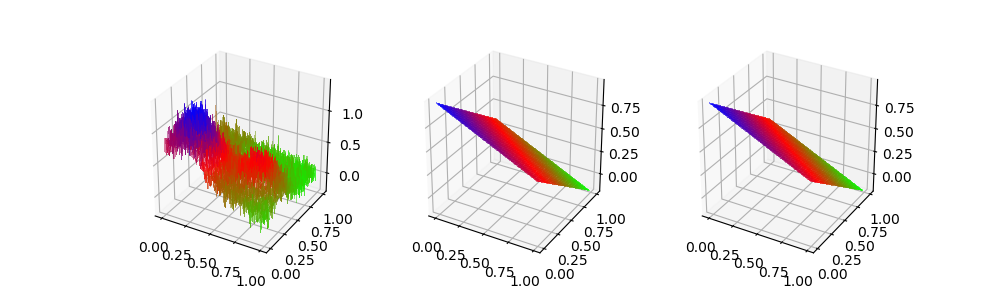
\includegraphics[width=1\linewidth]{images/surf/fake_linear_p01_n100.png}
  %\caption{}
  %\label{fig:v_x}
\end{subfigure}
\begin{subfigure}{\textwidth}
  \centering
  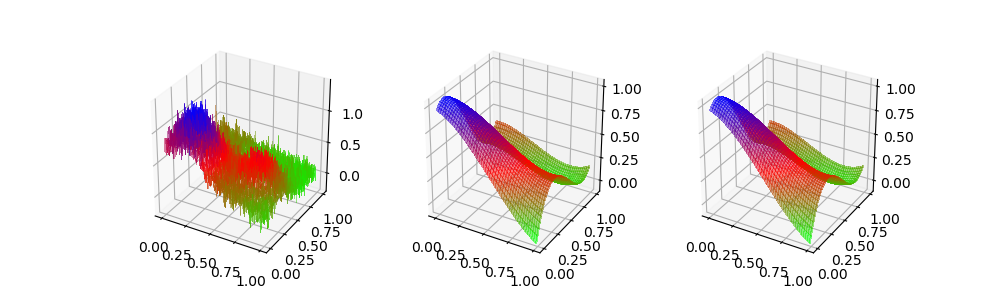
\includegraphics[width=1\linewidth]{images/surf/fake_linear_p03_n100.png}
  %\caption{}
  %\label{fig:vb_x}
\end{subfigure}
\begin{subfigure}{\textwidth}
  \centering
  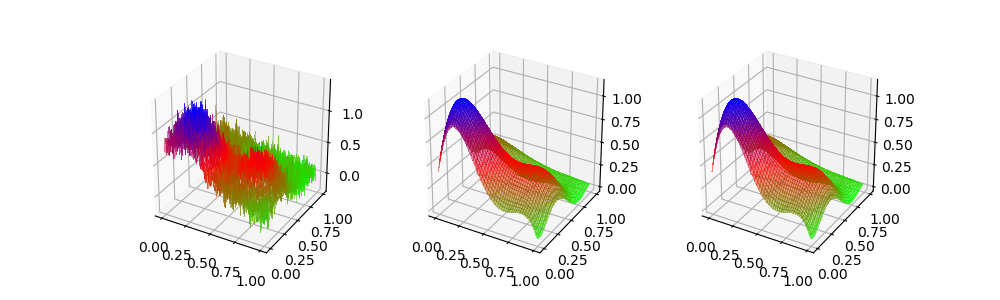
\includegraphics[width=1\linewidth]{images/surf/fake_linear_p05_n100.png}
  %\caption{}
  %\label{fig:v_x}
\end{subfigure}
\begin{subfigure}{\textwidth}
  \centering
  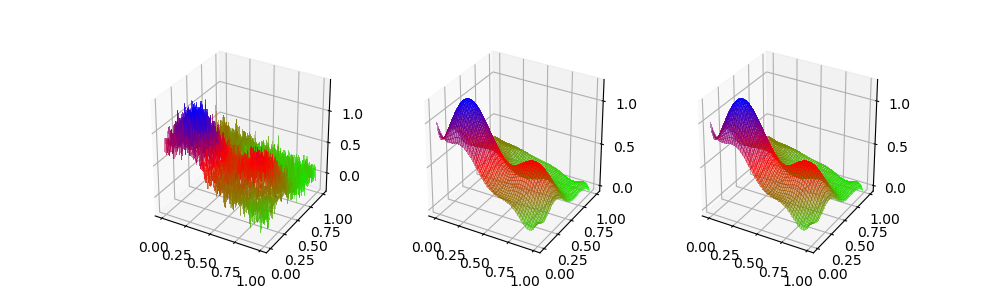
\includegraphics[width=1\linewidth]{images/surf/fake_linear_p08_n100.png}
  %\caption{}
  %\label{fig:v_x}
\end{subfigure}
\caption{The 3D visualisation of the noisy data set (left column) and the predicted surface via Lasso regression (right column) for polynomials 1, 3, 5 and 8 (from top to bottom). Grid is $100\times100$ points.}
\label{fig:linear-surf2}
\end{figure}
 
  \begin{figure}[!ht]
\begin{subfigure}{\textwidth}
  \centering
  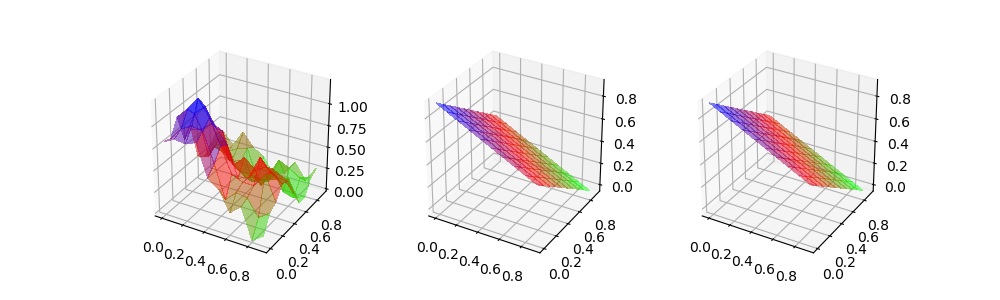
\includegraphics[width=1\linewidth]{images/surf/fake_ridge_p01_n10.png}
  %\caption{}
  %\label{fig:v_x}
\end{subfigure}
\begin{subfigure}{\textwidth}
  \centering
  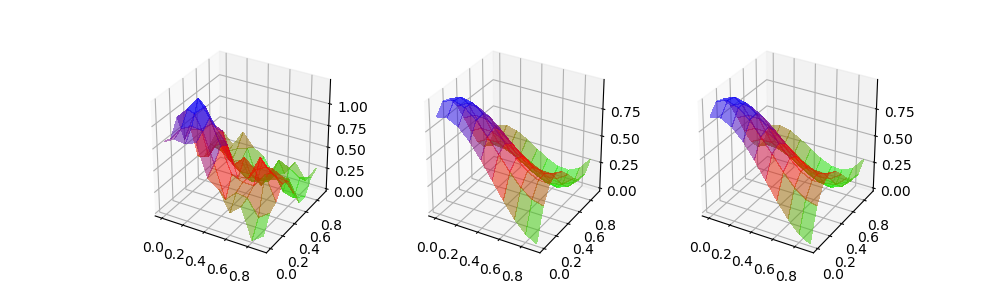
\includegraphics[width=1\linewidth]{images/surf/fake_ridge_p03_n10.png}
  %\caption{}
  %\label{fig:vb_x}
\end{subfigure}
\begin{subfigure}{\textwidth}
  \centering
  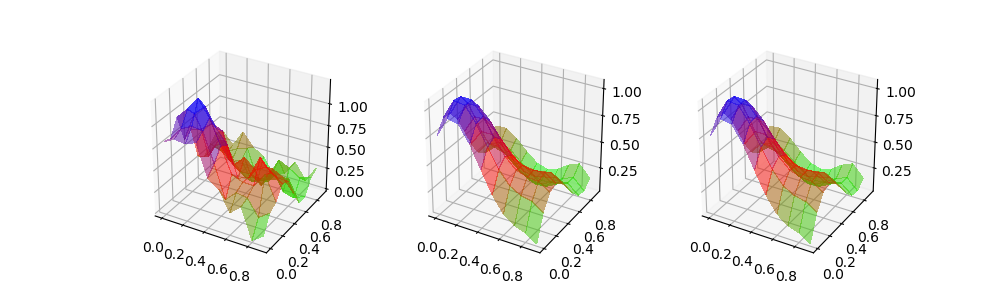
\includegraphics[width=1\linewidth]{images/surf/fake_ridge_p05_n10.png}
  %\caption{}
  %\label{fig:v_x}
\end{subfigure}
\begin{subfigure}{\textwidth}
  \centering
  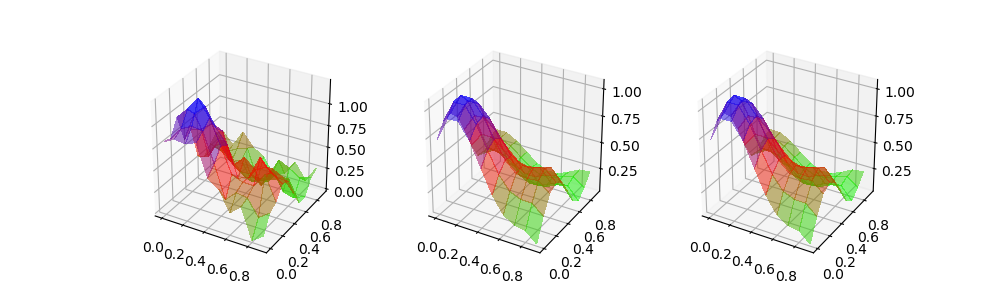
\includegraphics[width=1\linewidth]{images/surf/fake_ridge_p08_n10.png}
  %\caption{}
  %\label{fig:v_x}
\end{subfigure}
\caption{The 3D visualisation of the noisy data set (left column) and the predicted surface via Ridge regression (right column) for polynomials 1, 3, 5 and 8 (from top to bottom). Grid is $10\times10$ points and $\lambda = 0.0001$.}
\label{fig:ridge-surf1}
\end{figure}

 \begin{figure}[!ht]
\begin{subfigure}{\textwidth}
  \centering
  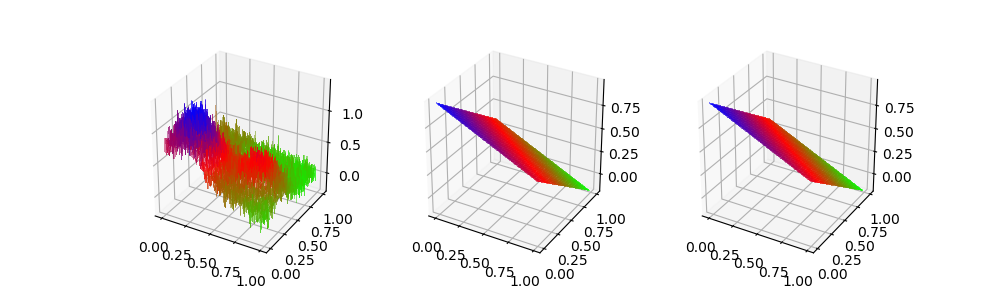
\includegraphics[width=1\linewidth]{images/surf/fake_ridge_p01_n100.png}
  %\caption{}
  %\label{fig:v_x}
\end{subfigure}
\begin{subfigure}{\textwidth}
  \centering
  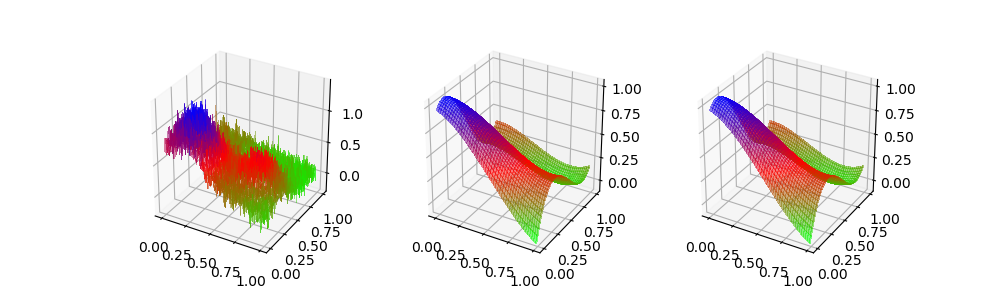
\includegraphics[width=1\linewidth]{images/surf/fake_ridge_p03_n100.png}
  %\caption{}
  %\label{fig:vb_x}
\end{subfigure}
\begin{subfigure}{\textwidth}
  \centering
  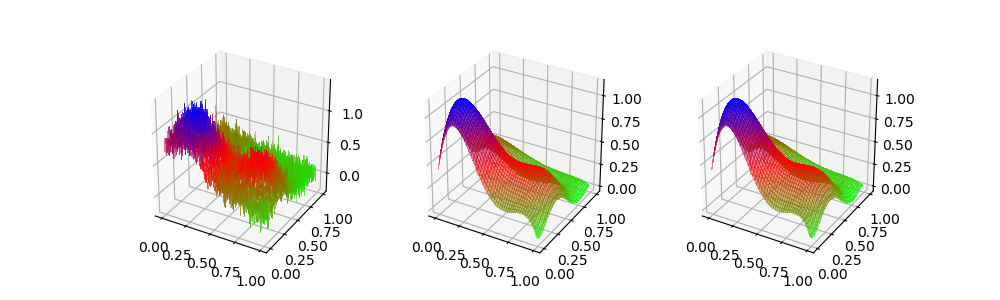
\includegraphics[width=1\linewidth]{images/surf/fake_ridge_p05_n100.png}
  %\caption{}
  %\label{fig:v_x}
\end{subfigure}
\begin{subfigure}{\textwidth}
  \centering
  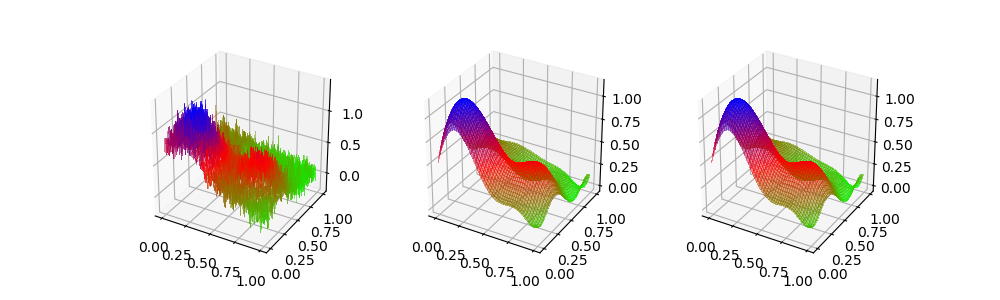
\includegraphics[width=1\linewidth]{images/surf/fake_ridge_p08_n100.png}
  %\caption{}
  %\label{fig:v_x}
\end{subfigure}
\caption{The 3D visualisation of the noisy data set (left column) and the predicted surface via Ridge regression (right column) for polynomials 1, 3, 5 and 8 (from top to bottom). Grid is $100\times100$ points and $\lambda = 0.0001$.}
\label{fig:ridge-surf2}
\end{figure}
 
\begin{figure}[!ht]
\begin{subfigure}{\textwidth}
  \centering
  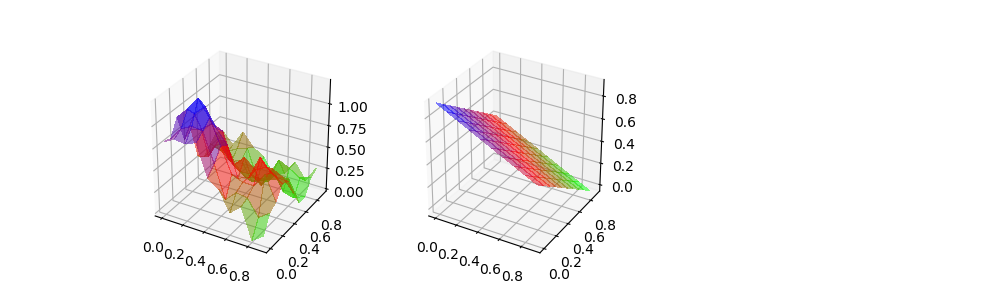
\includegraphics[width=1\linewidth]{images/surf/fake_lasso_p01_n10.png}
  %\caption{}
  %\label{fig:v_x}
\end{subfigure}
\begin{subfigure}{\textwidth}
  \centering
  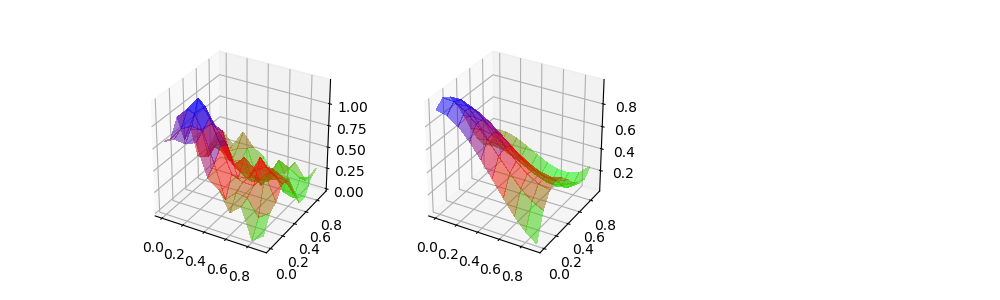
\includegraphics[width=1\linewidth]{images/surf/fake_lasso_p03_n10.png}
  %\caption{}
  %\label{fig:vb_x}
\end{subfigure}
\begin{subfigure}{\textwidth}
  \centering
  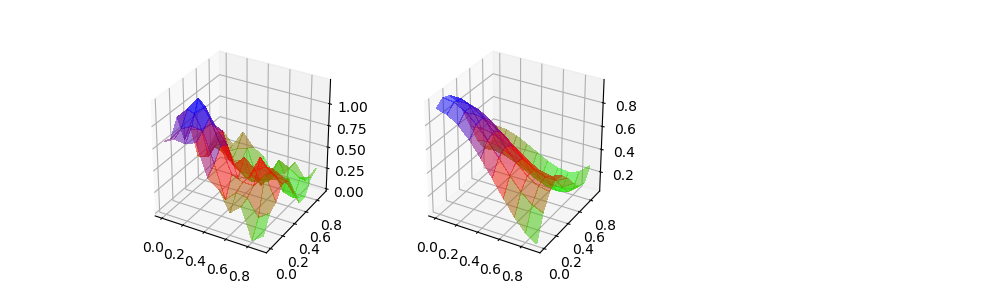
\includegraphics[width=1\linewidth]{images/surf/fake_lasso_p05_n10.png}
  %\caption{}
  %\label{fig:v_x}
\end{subfigure}
\begin{subfigure}{\textwidth}
  \centering
  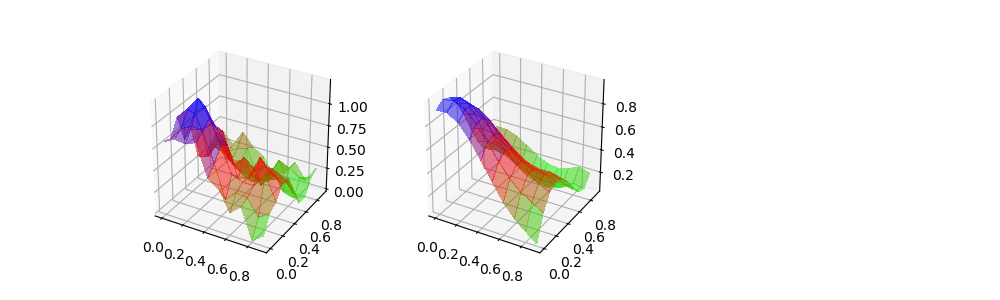
\includegraphics[width=1\linewidth]{images/surf/fake_lasso_p08_n10.png}
  %\caption{}
  %\label{fig:v_x}
\end{subfigure}
\caption{The 3D visualisation of the noisy data set (left column) and the predicted surface via Lasso regression (right column) for polynomials 1, 3, 5 and 8 (from top to bottom). Grid is $10\times10$ points and $\lambda = 0.0001$.}
\label{fig:lasso-surf1}
\end{figure}

\begin{figure}[!ht]
\begin{subfigure}{\textwidth}
  \centering
  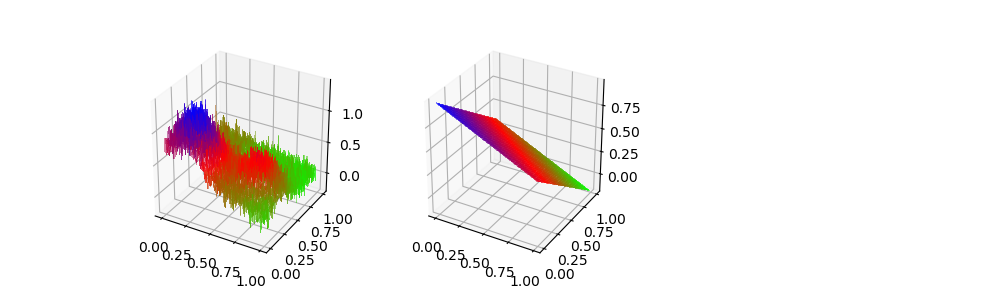
\includegraphics[width=1\linewidth]{images/surf/fake_lasso_p01_n100.png}
  %\caption{}
  %\label{fig:v_x}
\end{subfigure}
\begin{subfigure}{\textwidth}
  \centering
  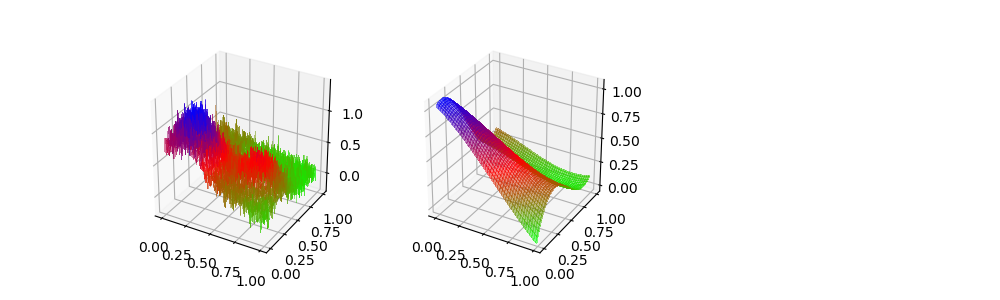
\includegraphics[width=1\linewidth]{images/surf/fake_lasso_p03_n100.png}
  %\caption{}
  %\label{fig:vb_x}
\end{subfigure}
\begin{subfigure}{\textwidth}
  \centering
  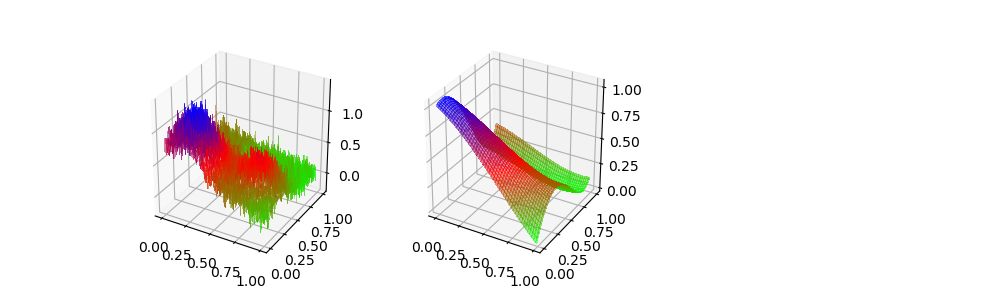
\includegraphics[width=1\linewidth]{images/surf/fake_lasso_p05_n100.png}
  %\caption{}
  %\label{fig:v_x}
\end{subfigure}
\begin{subfigure}{\textwidth}
  \centering
  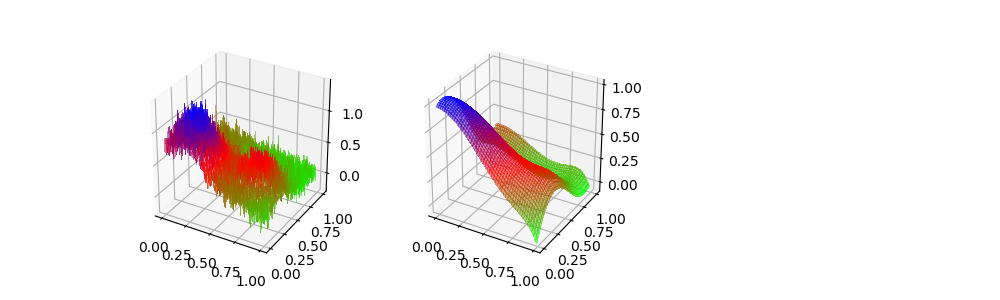
\includegraphics[width=1\linewidth]{images/surf/fake_lasso_p08_n100.png}
  %\caption{}
  %\label{fig:v_x}
\end{subfigure}
\caption{The 3D visualisation of the noisy data set (left column) and the predicted surface via Lasso regression (right column) for polynomials 1, 3, 5 and 8 (from top to bottom). Grid is $100\times100$ points and $\lambda = 0.0001$.}
\label{fig:lasso-surf2}
\end{figure}

%%%%%%%%%%%%%%%%%%%%%%%%%%%%%%%%%%%%%%%%%%%%%%%%%%%%%%%%%%%%%%%%%%%%%%%%%%%%%%%%%%%%%
% betas
%%%%%%%%%%%%%%%%%%%%%%%%%%%%%%%%%%%%%%%%%%%%%%%%%%%%%%%%%%%%%%%%%%%%%%%%%%%%%%%%%%%%%

\begin{figure}[!ht]
\begin{subfigure}{\textwidth}
  \centering
  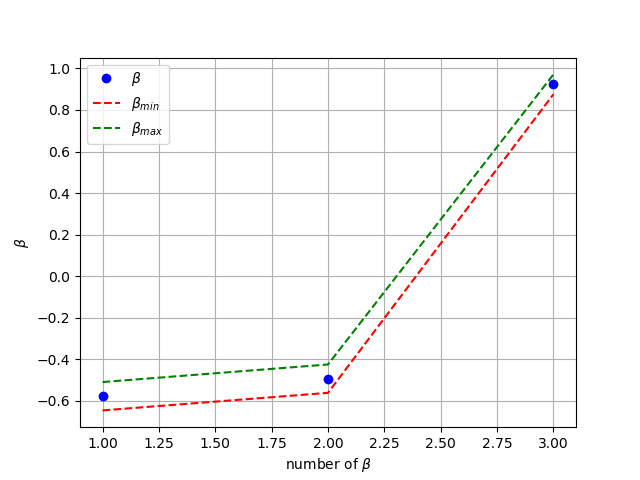
\includegraphics[width=0.5\linewidth]{images/betas/fake_linear_beta_p01_n10.png}
  %\caption{}
  %\label{fig:v_x}
\end{subfigure}
\begin{subfigure}{\textwidth}
  \centering
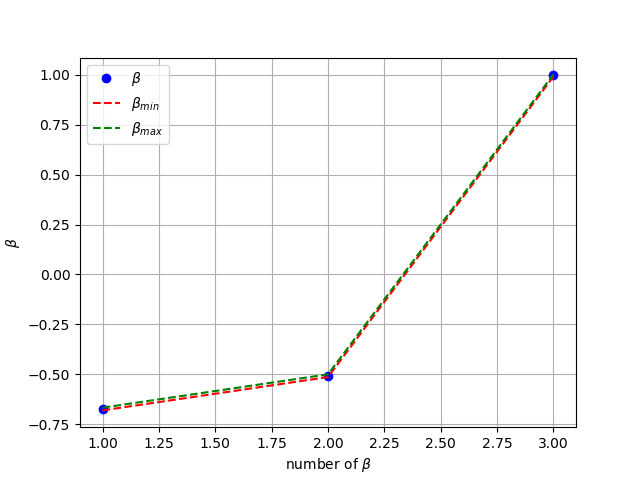
\includegraphics[width=0.5\linewidth]{images/betas/fake_linear_beta_p01_n100.png}
  %\caption{}
  %\label{fig:vb_x}
\end{subfigure}
\begin{subfigure}{\textwidth}
  \centering
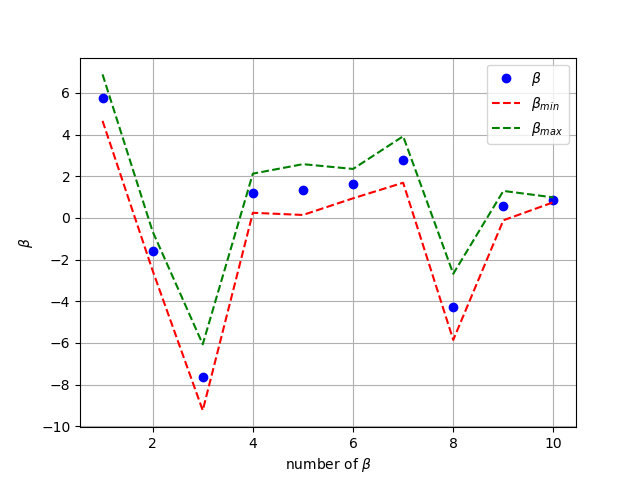
\includegraphics[width=0.5\linewidth]{images/betas/fake_linear_beta_p03_n10.png}
  %\caption{}
  %\label{fig:v_x}
\end{subfigure}
\begin{subfigure}{\textwidth}
  \centering
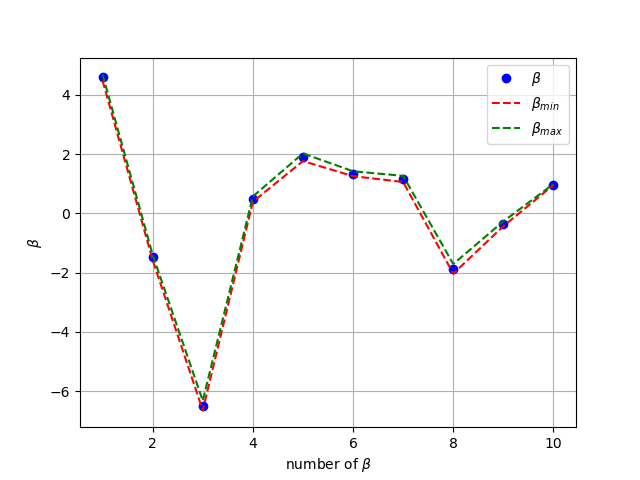
\includegraphics[width=0.5\linewidth]{images/betas/fake_linear_beta_p03_n100.png}
  %\caption{}
  %\label{fig:v_x}
\end{subfigure}
\begin{subfigure}{\textwidth}
  \centering
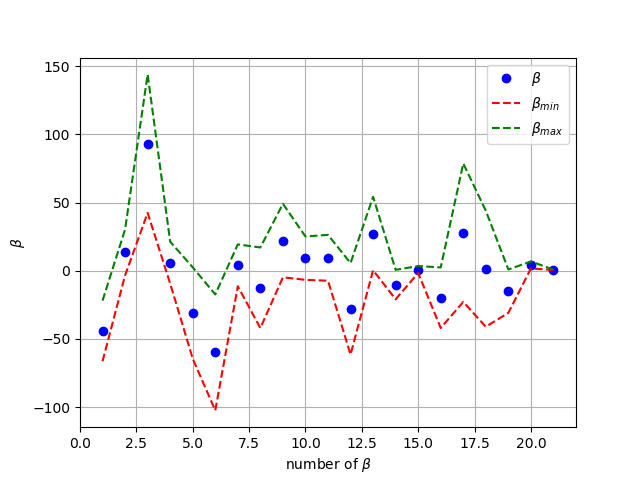
\includegraphics[width=0.5\linewidth]{images/betas/fake_linear_beta_p05_n10.png}
  %\caption{}
  %\label{fig:v_x}
\end{subfigure}
\begin{subfigure}{\textwidth}
  \centering
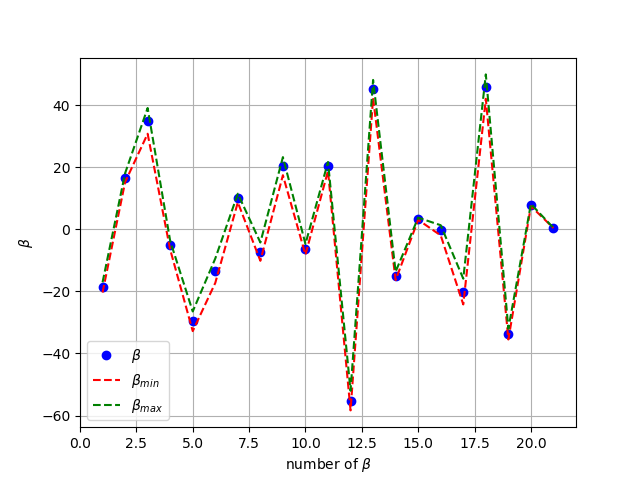
\includegraphics[width=0.5\linewidth]{images/betas/fake_linear_beta_p05_n100.png}
  %\caption{}
  %\label{fig:v_x}
\end{subfigure}
\begin{subfigure}{\textwidth}
  \centering
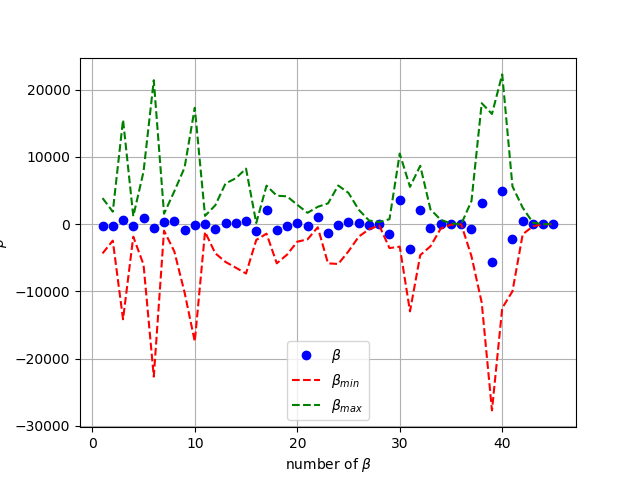
\includegraphics[width=0.5\linewidth]{images/betas/fake_linear_beta_p08_n10.png}
  %\caption{}
  %\label{fig:v_x}
\end{subfigure}
\begin{subfigure}{\textwidth}
  \centering
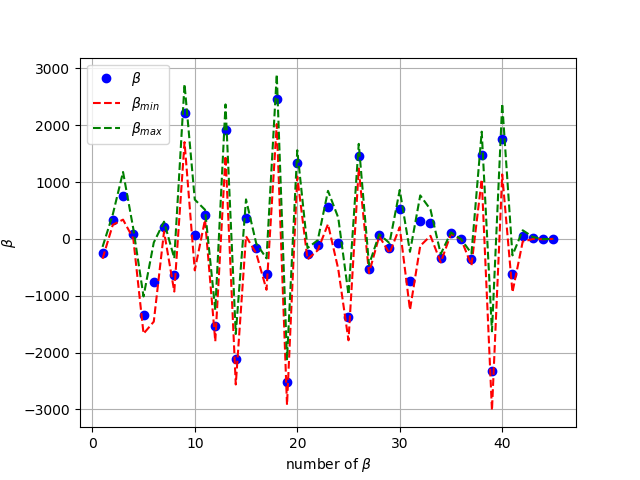
\includegraphics[width=0.5\linewidth]{images/betas/fake_linear_beta_p08_n100.png}
  %\caption{}
  %\label{fig:v_x}
\end{subfigure}
\caption{Manually calculated parameters $\beta$ of Linear Regression model for polynomials 1, 3, 5 and 8 (from top to bottom) on the grids $10\times10$ (left column) and $100\times100$ (right column) points.}
\label{fig:linear-beta}
\end{figure}

\begin{figure}[!ht]
\begin{subfigure}{\textwidth}
  \centering
  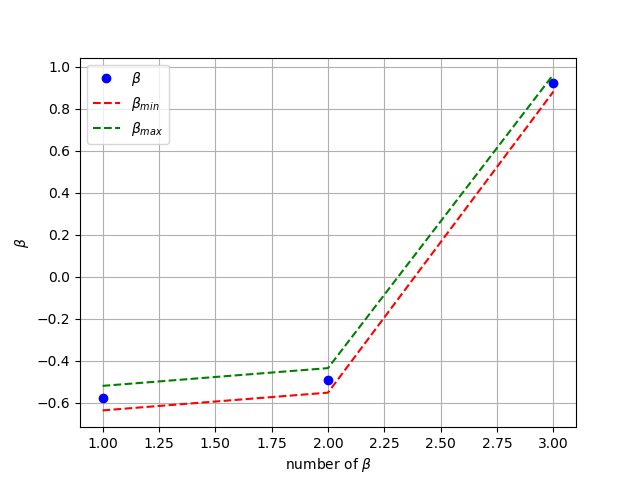
\includegraphics[width=0.5\linewidth]{images/betas/fake_ridge_beta_p01_n10.png}
  %\caption{}
  %\label{fig:v_x}
\end{subfigure}
\begin{subfigure}{\textwidth}
  \centering
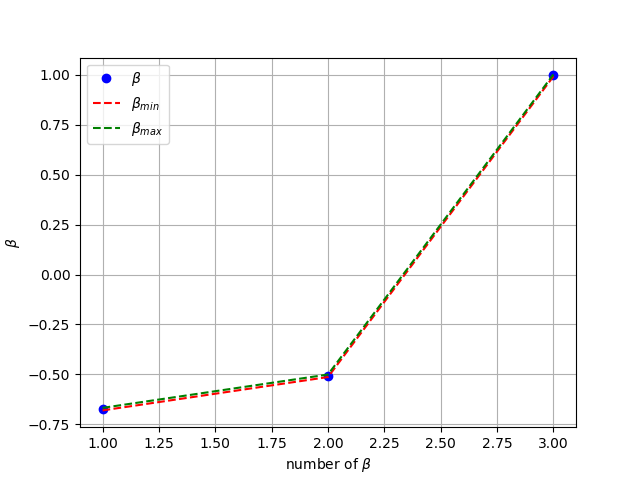
\includegraphics[width=0.5\linewidth]{images/betas/fake_ridge_beta_p01_n100.png}
  %\caption{}
  %\label{fig:vb_x}
\end{subfigure}
\begin{subfigure}{\textwidth}
  \centering
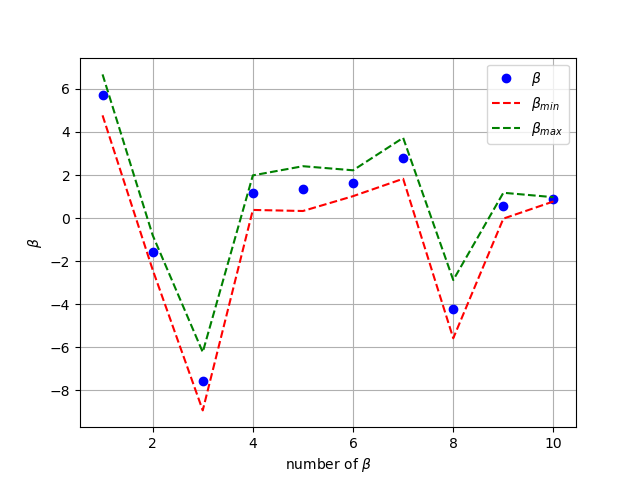
\includegraphics[width=0.5\linewidth]{images/betas/fake_ridge_beta_p03_n10.png}
  %\caption{}
  %\label{fig:v_x}
\end{subfigure}
\begin{subfigure}{\textwidth}
  \centering
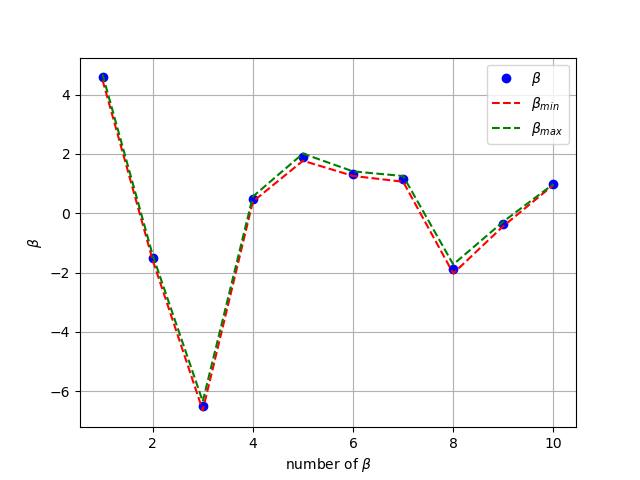
\includegraphics[width=0.5\linewidth]{images/betas/fake_ridge_beta_p03_n100.png}
  %\caption{}
  %\label{fig:v_x}
\end{subfigure}
\begin{subfigure}{\textwidth}
  \centering
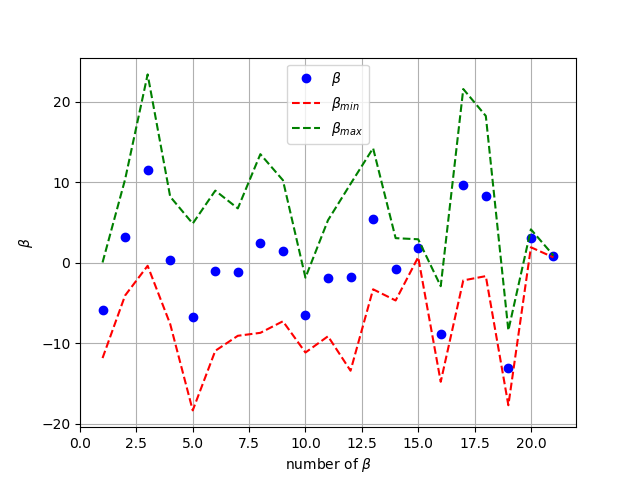
\includegraphics[width=0.5\linewidth]{images/betas/fake_ridge_beta_p05_n10.png}
  %\caption{}
  %\label{fig:v_x}
\end{subfigure}
\begin{subfigure}{\textwidth}
  \centering
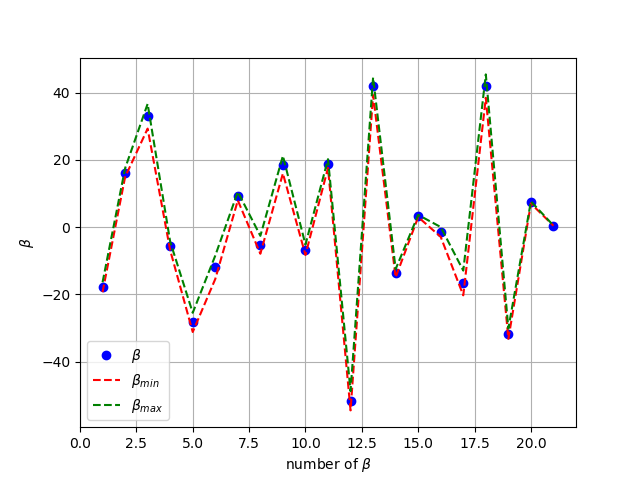
\includegraphics[width=0.5\linewidth]{images/betas/fake_ridge_beta_p05_n100.png}
  %\caption{}
  %\label{fig:v_x}
\end{subfigure}
\begin{subfigure}{\textwidth}
  \centering
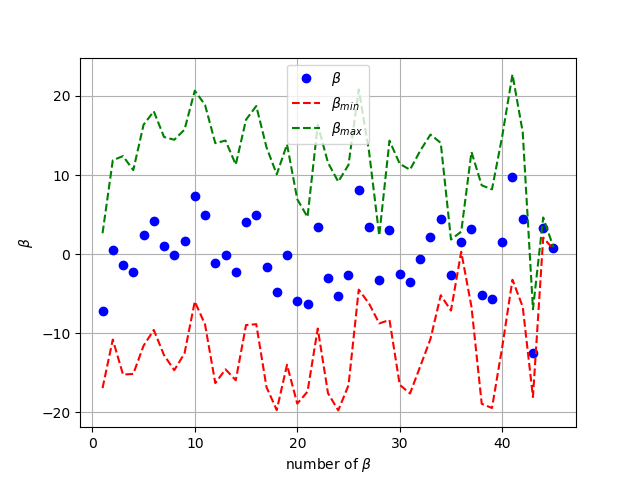
\includegraphics[width=0.5\linewidth]{images/betas/fake_ridge_beta_p08_n10.png}
  %\caption{}
  %\label{fig:v_x}
\end{subfigure}
\begin{subfigure}{\textwidth}
  \centering
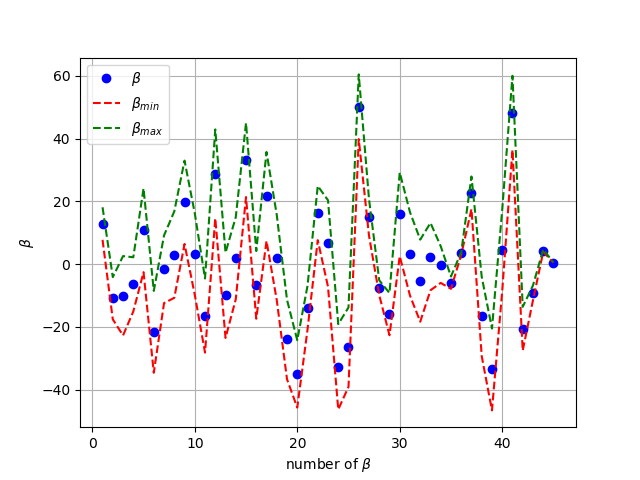
\includegraphics[width=0.5\linewidth]{images/betas/fake_ridge_beta_p08_n100.png}
  %\caption{}
  %\label{fig:v_x}
\end{subfigure}
\caption{Manually calculated parameters $\beta$ of Ridge Regression model for polynomials 1, 3, 5 and 8 (from top to bottom) on the grids $10\times10$ (left column) and $100\times100$ (right column) points. $\lambda = 0.0001$.}
\label{fig:ridge-beta}
\end{figure}

The corresponding beta parameters for Linear and Ridge regressions are plotted on figures \ref{fig:linear-beta} and \ref{fig:ridge-beta}. The left column is calculated for the $10\times10$ grid, whereas the right one has $100\times100$ points. In my opinion, it is clear from these plots, that the more points we have in the data set, the less uncertain we be about our model parameters.

Unfortunately, all these values cannot say for sure whether we will fit future data sets correctly (our main goal is to create such model) or not. That is why, as was discussed in the previous sections, we need to consider a resampling techniques. 

 \subsubsection{Resampling techniques: Bias-variance tradeoff}
 
 In section \ref{sec:formalism} I have described implementation of kFold Cross Validation Algorithm (with $k=5$). The part of the code rsponsible for it is the only part so far which is using  Parallelization with joblib to speed-up the process.
 
 Figures \ref{fig:linear-mse}-\ref{fig:lasso-mse} shows the MSEs for the training and test data sets respectively for several different grids as a function of polynomial degree (model complexity). The bias-variance trade-off is evident on the top plots (for each of the model). With lesser amount of points it becomes harder to fit the data, that is why the test curve diverges from the train one starting from polynomial of degree 3. 
 
 Figures \ref{fig:ridge-mse}-\ref{fig:lasso-mse} also shows the dependence on the hyper parameter for each regression type. As we can see, the smaller $\lambda$ becomes, the slopes are to the ones computed with OLS. Conversely, the increase in lambda parameter, will make the slope more flat, and that is because if we set $\lambda\rightarrow\infty$, $\beta=0$.
 
 Figures \ref{fig:linear-bias}-\ref{fig:lasso-bias} are plotting bias and varianse of the testing data set, resulted with kFold CV. The reason why bias is the straight line is unclear to me. Also, although variance is increasing with the model complexity, as it should, I don't really understand why it reaches some constant slope and stays there. Unfortunately, I couldn't resolve the issue no matter how hard I tried, and so, eventually, I decided to let it be.
 
 %%%%%%%%%%%%%%%%%%%%%%%%%%%%%%%%%%%%%%%%%%%%%%%%%%%%%%%%%%%%%%%%%%%%%%%%%%%%%%%%%%%%%
 % MSE
 %%%%%%%%%%%%%%%%%%%%%%%%%%%%%%%%%%%%%%%%%%%%%%%%%%%%%%%%%%%%%%%%%%%%%%%%%%%%%%%%%%%%%
\begin{figure}[!htbp]
\begin{subfigure}{\textwidth}
  \centering
  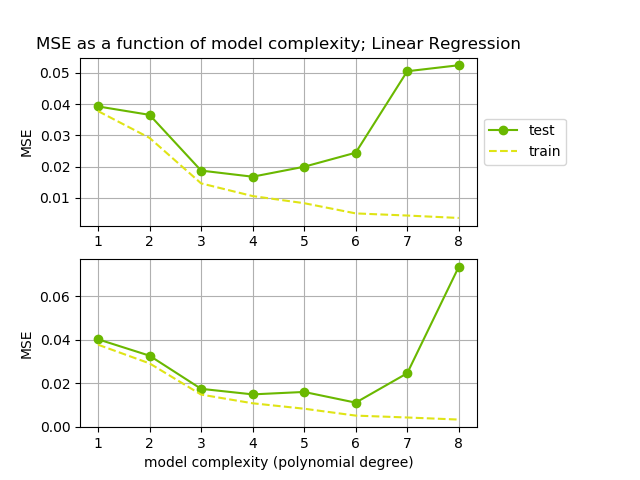
\includegraphics[width=0.55\linewidth]{images/mse/fake_linear_mse_p08_n10.png}
  %\caption{$10\times10$}
  %\label{fig:v_x}
\end{subfigure}
\begin{subfigure}{\textwidth}
  \centering
  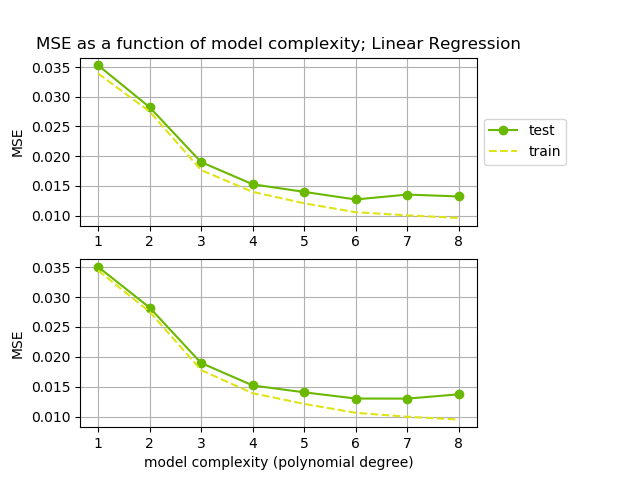
\includegraphics[width=0.55\linewidth]{images/mse/fake_linear_mse_p08_n21.png}
  %\caption{$21\times21$}
  %\label{fig:vb_x}
\end{subfigure}
\begin{subfigure}{\textwidth}
  \centering
  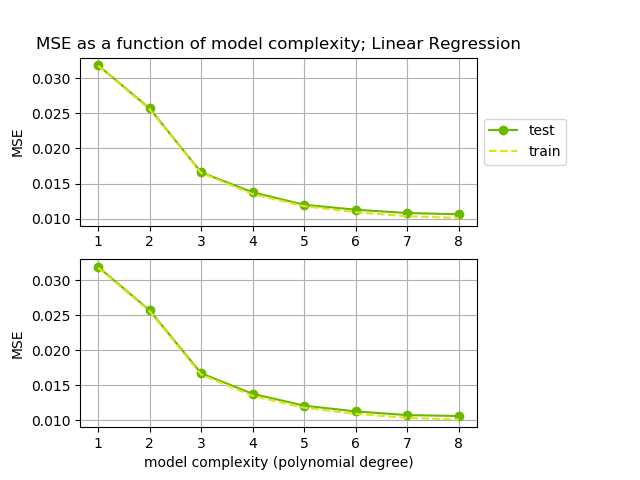
\includegraphics[width=0.55\linewidth]{images/mse/fake_linear_mse_p08_n50.png}
  %\caption{$50\times50$}
  %\label{fig:vb_x}
\end{subfigure}
\begin{subfigure}{\textwidth}
  \centering
  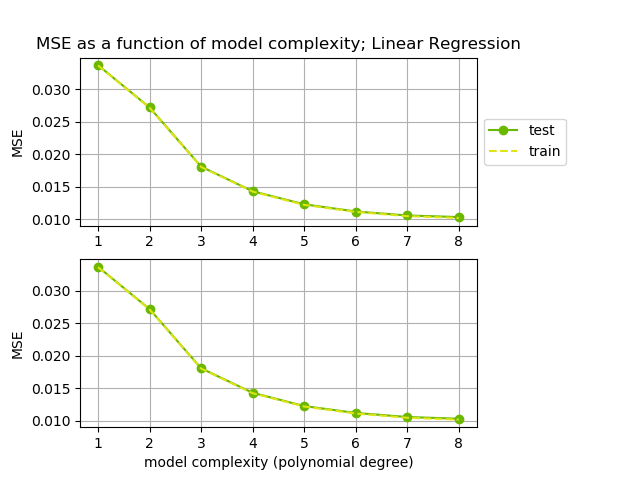
\includegraphics[width=0.55\linewidth]{images/mse/fake_linear_mse_p08_n100.png}
  %\caption{$100\times100$}
  %\label{fig:vb_x}
\end{subfigure}
\caption{MSE plot of train and test data sets as a function of model complexity (polynomial degree) calculated via Linear Regression for several different grids: $10\times10$ (top left), $21\times21$ (top right), $50\times50$ (bottom left), $100\times100$ (bottom right).}
\label{fig:linear-mse}
\end{figure}

\begin{figure}[!htbp]
\begin{subfigure}{\textwidth}
  \centering
  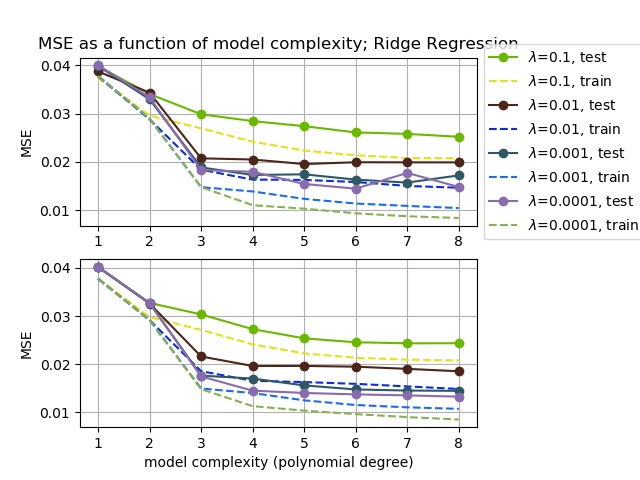
\includegraphics[width=0.55\linewidth]{images/mse/fake_ridge_mse_p08_n10.png}
  %\caption{$10\times10$}
  %\label{fig:v_x}
\end{subfigure}
\begin{subfigure}{\textwidth}
  \centering
  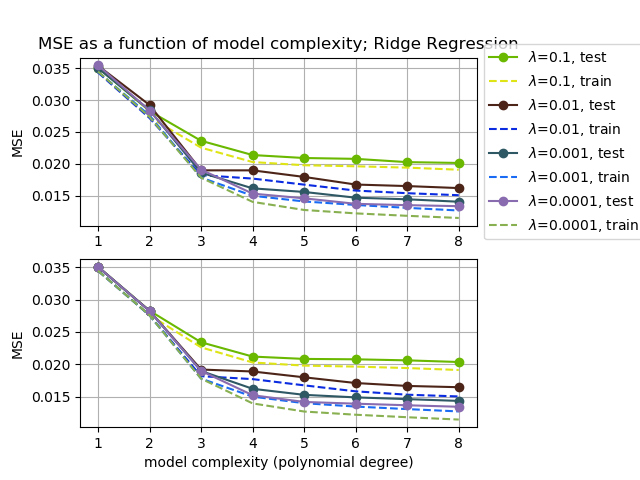
\includegraphics[width=0.55\linewidth]{images/mse/fake_ridge_mse_p08_n21.png}
  %\caption{$21\times21$}
  %\label{fig:vb_x}
\end{subfigure}
\begin{subfigure}{\textwidth}
  \centering
  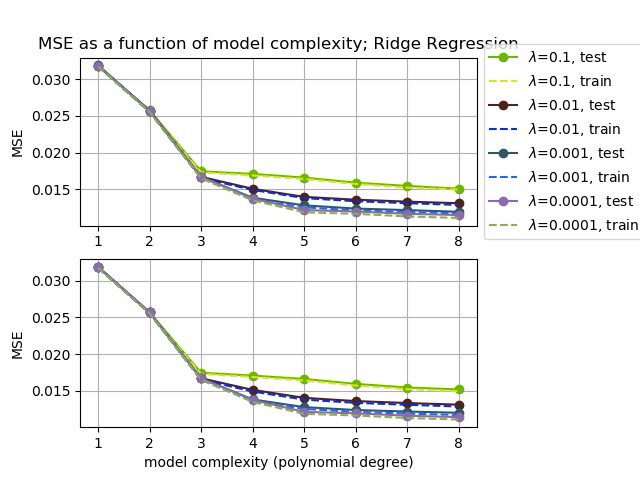
\includegraphics[width=0.55\linewidth]{images/mse/fake_ridge_mse_p08_n50.png}
  %\caption{$50\times50$}
  %\label{fig:vb_x}
\end{subfigure}
\begin{subfigure}{\textwidth}
  \centering
  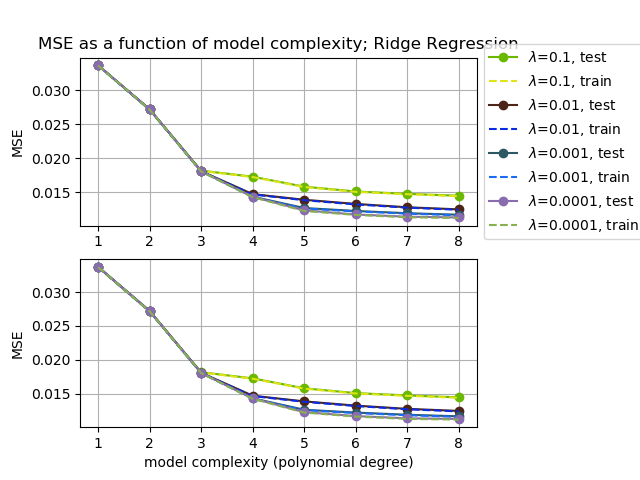
\includegraphics[width=0.55\linewidth]{images/mse/fake_ridge_mse_p08_n100.png}
  %\caption{$100\times100$}
  %\label{fig:vb_x}
\end{subfigure}
\caption{MSE plot of train and test data sets as a function of model complexity (polynomial degree) calculated via Ridge Regression for several different grids: $10\times10$ (top left), $21\times21$ (top right), $50\times50$ (bottom left), $100\times100$ (bottom right). $\lambda_i = 0.1$, $0.01$ and $0.0001$.}
\label{fig:ridge-mse}
\end{figure}

\begin{figure}[!htbp]
\begin{subfigure}{\textwidth}
  \centering
  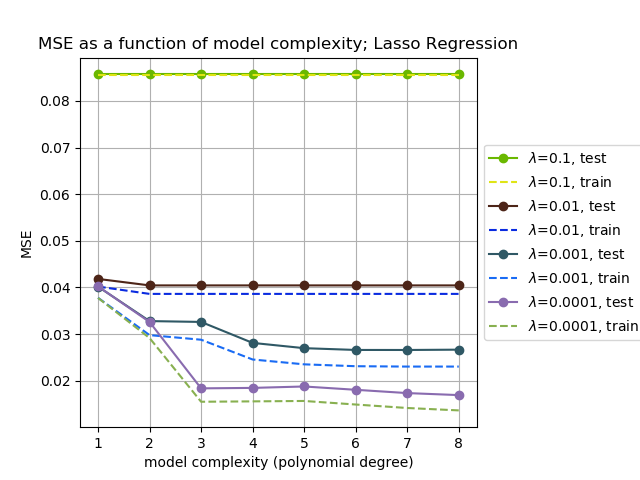
\includegraphics[width=0.55\linewidth]{images/mse/fake_lasso_mse_p08_n10.png}
  %\caption{$10\times10$}
  %\label{fig:v_x}
\end{subfigure}
\begin{subfigure}{\textwidth}
  \centering
  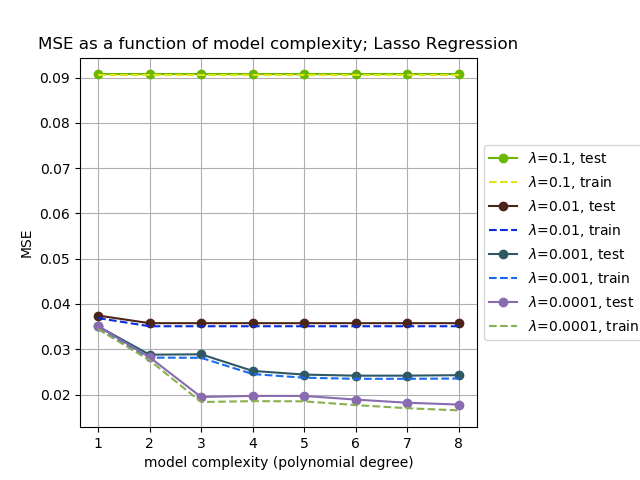
\includegraphics[width=0.55\linewidth]{images/mse/fake_lasso_mse_p08_n21.png}
  %\caption{$21\times21$}
  %\label{fig:vb_x}
\end{subfigure}
\begin{subfigure}{\textwidth}
  \centering
  \includegraphics[width=0.55\linewidth]{images/mse/fake_lasso_mse_p08_n50.png}
  %\caption{$50\times50$}
  %\label{fig:vb_x}
\end{subfigure}
\begin{subfigure}{\textwidth}
  \centering
  \includegraphics[width=0.55\linewidth]{images/mse/fake_lasso_mse_p08_n100.png}
  %\caption{$100\times100$}
  %\label{fig:vb_x}
\end{subfigure}
\caption{MSE plot of train and test data sets as a function of model complexity (polynomial degree) calculated via Lasso Regression for several different grids: $10\times10$ (top left), $21\times21$ (top right), $50\times50$ (bottom left), $100\times100$ (bottom right). $\lambda_i = 0.1$, $0.01$ and $0.0001$.}
\label{fig:lasso-mse}
\end{figure}

 %%%%%%%%%%%%%%%%%%%%%%%%%%%%%%%%%%%%%%%%%%%%%%%%%%%%%%%%%%%%%%%%%%%%%%%%%%%%%%%%%%%%%
 % Bias/Variance trade-off
 %%%%%%%%%%%%%%%%%%%%%%%%%%%%%%%%%%%%%%%%%%%%%%%%%%%%%%%%%%%%%%%%%%%%%%%%%%%%%%%%%%%%%

 \begin{figure}[!ht]
\begin{subfigure}{\textwidth}
  \centering
  \includegraphics[width=0.55\linewidth]{images/bias_var/fake_linear_bv_p08_n10.png}
  %\caption{$10\times10$}
  %\label{fig:v_x}
\end{subfigure}
\begin{subfigure}{\textwidth}
  \centering
  \includegraphics[width=0.55\linewidth]{images/bias_var/fake_linear_bv_p08_n21.png}
  %\caption{$21\times21$}
  %\label{fig:vb_x}
\end{subfigure}
\begin{subfigure}{\textwidth}
  \centering
  \includegraphics[width=0.55\linewidth]{images/bias_var/fake_linear_bv_p08_n50.png}
  %\caption{$50\times50$}
  %\label{fig:vb_x}
\end{subfigure}
\begin{subfigure}{\textwidth}
  \centering
  \includegraphics[width=0.55\linewidth]{images/bias_var/fake_linear_bv_p08_n100.png}
  %\caption{$100\times100$}
  %\label{fig:vb_x}
\end{subfigure}
\caption{Plot of Bias and Variance (to illustrate bias-variance trade-off) as a function of model complexity (polynomial degree) calculated via Linear Regression for several different grids: $10\times10$ (top left), $21\times21$ (top right), $50\times50$ (bottom left), $100\times100$ (bottom right). $\lambda_i = 0.1$, $0.01$ and $0.0001$.}
\label{fig:linear-bias}
\end{figure}

 \begin{figure}[!ht]
\begin{subfigure}{\textwidth}
  \centering
  \includegraphics[width=0.55\linewidth]{images/bias_var/fake_ridge_bv_p08_n10.png}
  %\caption{$10\times10$}
  %\label{fig:v_x}
\end{subfigure}
\begin{subfigure}{\textwidth}
  \centering
  \includegraphics[width=0.55\linewidth]{images/bias_var/fake_ridge_bv_p08_n21.png}
  %\caption{$21\times21$}
  %\label{fig:vb_x}
\end{subfigure}
\begin{subfigure}{\textwidth}
  \centering
  \includegraphics[width=0.55\linewidth]{images/bias_var/fake_ridge_bv_p08_n50.png}
  %\caption{$50\times50$}
  %\label{fig:vb_x}
\end{subfigure}
\begin{subfigure}{\textwidth}
  \centering
  \includegraphics[width=0.55\linewidth]{images/bias_var/fake_ridge_bv_p08_n100.png}
  %\caption{$100\times100$}
  %\label{fig:vb_x}
\end{subfigure}
\caption{Plot of Bias and Variance (to illustrate bias-variance trade-off) as a function of model complexity (polynomial degree) calculated via Ridge Regression for several different grids: $10\times10$ (top left), $21\times21$ (top right), $50\times50$ (bottom left), $100\times100$ (bottom right). $\lambda_i = 0.1$, $0.01$ and $0.0001$.}
\label{fig:ridge-bias}
\end{figure}


\begin{figure}[!ht]
\begin{subfigure}{\textwidth}
  \centering
  \includegraphics[width=0.55\linewidth]{images/bias_var/fake_lasso_bv_p08_n10.png}
  %\caption{$10\times10$}
  %\label{fig:v_x}
\end{subfigure}
\begin{subfigure}{\textwidth}
  \centering
  \includegraphics[width=0.55\linewidth]{images/bias_var/fake_lasso_bv_p08_n21.png}
  %\caption{$21\times21$}
  %\label{fig:vb_x}
\end{subfigure}
\begin{subfigure}{\textwidth}
  \centering
  \includegraphics[width=0.55\linewidth]{images/bias_var/fake_lasso_bv_p08_n50.png}
  %\caption{$50\times50$}
  %\label{fig:vb_x}
\end{subfigure}
\begin{subfigure}{\textwidth}
  \centering
  \includegraphics[width=0.55\linewidth]{images/bias_var/fake_lasso_bv_p08_n100.png}
  %\caption{$100\times100$}
  %\label{fig:vb_x}
\end{subfigure}
\caption{Plot of Bias and Variance (to illustrate bias-variance trade-off) as a function of model complexity (polynomial degree) calculated via Lasso Regression for several different grids: $10\times10$ (top left), $21\times21$ (top right), $50\times50$ (bottom left), $100\times100$ (bottom right). $\lambda_i = 0.1$, $0.01$ and $0.0001$.}
\label{fig:lasso-bias}
\end{figure}


 \subsection{Real Data}
 
For the real data set we need to repeat the same things we did for the fake one. However, here it is useful to take only a part of the terrain data to train and test your model on.
 
 The procedures for calculating values for real data set is the same as for the manually generated one. The only problem here is that to run the entire data set for 5 different consecutive polynomial degrees, took me about 7 hours. To be more precise, the console output showed:
 \begin{lstlisting}
-- Program finished at 26326.446545124054 sec --
\end{lstlisting}
Below I discuss this in a more detail.

\subsubsection{Entire Data set}

For this run, I am plotting the resulting fitted surfaces in figures \ref{fig:linear-surf-real}-\ref{fig:lasso-surf-real}. The entire file consists of $3601\times1801 = 6485401$ points in total. %For such a large system, overfitting is impossible to provoke, because both test set and train set will not reach the white noise threshold in the "near future". Thus, the slopes are identical for this polynomial degree.

Lets take a look for MSE resulting from Cross Validation - figures \ref{fig:linear-mse-real-all}-\ref{fig:lasso-mse-real-all}. As we can see, both test and training data sets in ideal sync, which tells us that the amount of points in the system is so large, that the slopes will not reach white noise threshold in the "near future".
Unfortunately, the Bias-Variance plots \ref{fig:real-bias-all} also shows the same weird behavior as with the pre-generated data set.

Now, I was not able to test the program for the larger polynomials, but I am confident enough to say it will not show any sigh of overfitting up to polynomial of degree 20.

The beta values with their confidence intervals are plotted in figures \ref{fig:linear-beta-real}-\ref{fig:ridge-beta-real}. Unfortunately, it is hard for me to tell whether these values are correct or not, or why is there this bump for the last coefficient looking on the plots themselves. My idea is that it is because I didn't normalize my data, before actually fitting it, but it is still needs to be tested.

\begin{figure}[!ht]
\begin{subfigure}{\textwidth}
  \centering
  \includegraphics[width=0.5\linewidth]{images/real/real_linear_beta_p01_nreal.png}
  %\caption{}
  %\label{fig:v_x}
\end{subfigure}
\begin{subfigure}{\textwidth}
  \centering
\includegraphics[width=0.5\linewidth]{images/real/real_ridge_beta_p02_nreal.png}
  %\caption{}
  %\label{fig:vb_x}
\end{subfigure}
\begin{subfigure}{\textwidth}
  \centering
\includegraphics[width=0.5\linewidth]{images/real/real_linear_beta_p03_nreal.png}
  %\caption{}
  %\label{fig:v_x}
\end{subfigure}
\begin{subfigure}{\textwidth}
  \centering
\includegraphics[width=0.5\linewidth]{images/real/real_ridge_beta_p04_nreal.png}
  %\caption{}
  %\label{fig:v_x}
\end{subfigure}
\begin{subfigure}{\textwidth}
  \centering
\includegraphics[width=0.5\linewidth]{images/real/real_linear_beta_p05_nreal.png}
  %\caption{}
  %\label{fig:v_x}
\end{subfigure}
\caption{Manually calculated parameters $\beta$ of Linear Regression model for polynomials 1, 2, 3, 4 and 5 (from top to bottom) on the entire data set ($3601\times1801 = 6485401$ points).}
\label{fig:linear-beta-real}
\end{figure}

\begin{figure}[!ht]
\begin{subfigure}{\textwidth}
  \centering
  \includegraphics[width=0.5\linewidth]{images/real/real_ridge_beta_p01_nreal.png}
  %\caption{}
  %\label{fig:v_x}
\end{subfigure}
\begin{subfigure}{\textwidth}
  \centering
\includegraphics[width=0.5\linewidth]{images/real/real_ridge_beta_p02_nreal.png}
  %\caption{}
  %\label{fig:vb_x}
\end{subfigure}
\begin{subfigure}{\textwidth}
  \centering
\includegraphics[width=0.5\linewidth]{images/real/real_ridge_beta_p03_nreal.png}
  %\caption{}
  %\label{fig:v_x}
\end{subfigure}
\begin{subfigure}{\textwidth}
  \centering
\includegraphics[width=0.5\linewidth]{images/real/real_ridge_beta_p04_nreal.png}
  %\caption{}
  %\label{fig:v_x}
\end{subfigure}
\begin{subfigure}{\textwidth}
  \centering
\includegraphics[width=0.5\linewidth]{images/real/real_ridge_beta_p05_nreal.png}
  %\caption{}
  %\label{fig:v_x}
\end{subfigure}
\caption{Manually calculated parameters $\beta$ of Linear Regression model for polynomials 1, 2, 3, 4 and 5 (from top to bottom) on the entire data set ($3601\times1801 = 6485401$ points). $\lambda=0.0001$}
\label{fig:ridge-beta-real}
\end{figure}

\begin{figure}[!ht]
\begin{subfigure}{\textwidth}
  \centering
  \includegraphics[width=0.7\linewidth]{images/real/real_linear_bv_p05_nreal.png}
  %\caption{$10\times10$}
  %\label{fig:v_x}
\end{subfigure}
\begin{subfigure}{\textwidth}
  \centering
  \includegraphics[width=0.7\linewidth]{images/real/real_ridge_bv_p05_nreal.png}
  %\caption{$21\times21$}
  %\label{fig:vb_x}
\end{subfigure}
\begin{subfigure}{\textwidth}
  \centering
  \includegraphics[width=0.7\linewidth]{images/real/real_lasso_bv_p05_nreal.png}
  %\caption{$50\times50$}
  %\label{fig:vb_x}
\end{subfigure}
\caption{Plot of Bias and Variance (to illustrate bias-variance trade-off) as a function of model complexity (polynomial degree) calculated via Linear, Ridge and Lasso Regressions (from top to bottom) for entire data set ($3601\times1801 = 6485401$ points). $\lambda_i = 0.1$, $0.01$ and $0.0001$.}
\label{fig:real-bias-all}
\end{figure}

Anyway, I think it is pretty safe to say that for the entire data set, the \textit{best optimal model will be OLS}.

\subsubsection{Portion of Dataset}

As, I've already stated, the last version of the program allows you to decide on which $\%$ of the data set to use. Following some of the students suggestions, I decided to use the $5\%$ of the entire data set, i.e. $181\times1801=325981$ points. Although, the total amount of points is significantly lesser, it is still pretty huge system to look into. 

As we saw, for the system of $10000$ ($100\times100$ grid), we start overfitting the model only at polynomial of 8 degree and higher. Now, we have 30 times more data points, which means we need to significantly increase the degree of polynomial to fit in.

I tried to run the code with max polynomial of 20. However, with the increase of polynomial degree, the model started to give completely incorrect results. For instance, figure \ref{fig:linear-surf-real-small} shows the 3d surface visualization for several different polynomials. Until polynomial of 7th degree, the Linear regression model was fitting perfectly, but as it clearly seen, we get completely incorrect results. Another indication of the wrong model - the negative $R^2$ values in the table \ref{table:all-mse2} below.

 \begin{figure}[ht]
\begin{subfigure}{\textwidth}
  \centering
  \includegraphics[width=1\linewidth]{images/real_part/real_linear_p03_nreal.png}
  %\caption{}
  %\label{fig:v_x}
\end{subfigure}
\begin{subfigure}{\textwidth}
  \centering
  \includegraphics[width=1\linewidth]{images/real_part/real_linear_p05_nreal.png}
  %\caption{}
  %\label{fig:vb_x}
\end{subfigure}
\begin{subfigure}{\textwidth}
  \centering
  \includegraphics[width=1\linewidth]{images/real_part/real_linear_p07_nreal.png}
  %\caption{}
  %\label{fig:v_x}
\end{subfigure}
\caption{The 3D visualisation of the $5\%$ of the real noisy data set (left column) and the predicted surface via Linear regression (right column) for polynomials 3, 5, 7 (from top to bottom).}
\label{fig:linear-surf-real-small}
\end{figure}

%%%%%%%%%%%%%%%%%%%%%%%%%%%%%%%%%%%%%%%%%%%%%%%%%%%%%%%%%%%%%%%%%%%%%%%%%%%%%%%%%%%%%
 % MSE
 %%%%%%%%%%%%%%%%%%%%%%%%%%%%%%%%%%%%%%%%%%%%%%%%%%%%%%%%%%%%%%%%%%%%%%%%%%%%%%%%%%%%%
\begin{figure}[ht]
\begin{subfigure}{\textwidth}
  \centering
  \includegraphics[width=0.55\linewidth]{images/real_part/real_linear_mse_p07_nreal.png}
  %\caption{$10\times10$}
  %\label{fig:v_x}
\end{subfigure}
\begin{subfigure}{\textwidth}
  \centering
  \includegraphics[width=0.55\linewidth]{images/real_part/real_ridge_mse_p07_nreal.png}
  %\caption{$21\times21$}
  %\label{fig:vb_x}
\end{subfigure}
\begin{subfigure}{\textwidth}
  \centering
  \includegraphics[width=0.55\linewidth]{images/real_part/real_lasso_mse_p07_nreal.png}
  %\caption{$50\times50$}
  %\label{fig:vb_x}
\end{subfigure}
\caption{MSE plot of train and test data sets as a function of model complexity (polynomial degree) calculated via Linear Ridge and Lasso Regression on the $5\%$ of th real data set (bottom right).}
\label{fig:linear-mse-real-small}
\end{figure}

The Cross Validation MSEs for test and train data sets for a given polynomial degree can be found in the plot \ref{fig:linear-mse-real-small}. Once again, we see that the two slopes are perfectly aligned which tells us we won't reach over fitting with this amount of points. So, my understanding is that I need to decrease the amount of points even further down. The bias and variance executes the same weird behavior as in the previous cases, so I do not show them here. The same goes for betas (although the plots and the values are available inside "/Output/" folder under appropriate name).


\begin{figure}[!ht]
\begin{subfigure}{\textwidth}
  \centering
  \includegraphics[width=0.55\linewidth]{images/mse/fake_linear_mse_p08_n10.png}
  %\caption{$10\times10$}
  %\label{fig:v_x}
\end{subfigure}
\begin{subfigure}{\textwidth}
  \centering
  \includegraphics[width=0.55\linewidth]{images/mse/fake_linear_mse_p08_n21.png}
  %\caption{$21\times21$}
  %\label{fig:vb_x}
\end{subfigure}
\begin{subfigure}{\textwidth}
  \centering
  \includegraphics[width=0.55\linewidth]{images/mse/fake_linear_mse_p08_n50.png}
  %\caption{$50\times50$}
  %\label{fig:vb_x}
\end{subfigure}
\begin{subfigure}{\textwidth}
  \centering
  \includegraphics[width=0.55\linewidth]{images/mse/fake_linear_mse_p08_n100.png}
  %\caption{$100\times100$}
  %\label{fig:vb_x}
\end{subfigure}
\caption{MSE plot of train and test data sets as a function of model complexity (polynomial degree) calculated via Linear Regression for several different grids: $10\times10$ (top left), $21\times21$ (top right), $50\times50$ (bottom left), $100\times100$ (bottom right).}
\label{fig:linear-mse-real-all}
\end{figure}

\begin{figure}[!ht]
\begin{subfigure}{\textwidth}
  \centering
  \includegraphics[width=0.55\linewidth]{images/mse/fake_ridge_mse_p08_n10.png}
  %\caption{$10\times10$}
  %\label{fig:v_x}
\end{subfigure}
\begin{subfigure}{\textwidth}
  \centering
  \includegraphics[width=0.55\linewidth]{images/mse/fake_ridge_mse_p08_n21.png}
  %\caption{$21\times21$}
  %\label{fig:vb_x}
\end{subfigure}
\begin{subfigure}{\textwidth}
  \centering
  \includegraphics[width=0.55\linewidth]{images/mse/fake_ridge_mse_p08_n50.png}
  %\caption{$50\times50$}
  %\label{fig:vb_x}
\end{subfigure}
\begin{subfigure}{\textwidth}
  \centering
  \includegraphics[width=0.55\linewidth]{images/mse/fake_ridge_mse_p08_n100.png}
  %\caption{$100\times100$}
  %\label{fig:vb_x}
\end{subfigure}
\caption{MSE plot of train and test data sets as a function of model complexity (polynomial degree) calculated via Ridge Regression for several different grids: $10\times10$ (top left), $21\times21$ (top right), $50\times50$ (bottom left), $100\times100$ (bottom right). $\lambda_i = 0.1$, $0.01$ and $0.0001$.}
\label{fig:ridge-mse-real-all}
\end{figure}


\begin{table}[h!]
\begin{tabular}{ |p{2cm}|p{3cm}|p{3cm}|p{3cm}|p{3cm}|  }
 \hline
 \multicolumn{5}{|c|}{Regression Type} \\
 \hline
 Polynomial \newline Degree & Linear \newline MSE, $R^2$ & Ridge \newline MSE, $R^2$ & Lasso \newline MSE, $R^2$  & Type\\
 \hline
 1 & 761.9179, 0.9720 \newline 761.9179, 0.9720 & 761.917, 0.972 \newline 761.917, 0.972 & 761.9179, 0.9720 & Scikit Learn \newline Manual\\
 \hline
 2 & 659.9133, 0.9757 \newline 659.9133, 0.9757  & 659.9133, 0.9757 \newline 659.9133, 0.9757 & 659.9133, 0.975 & Scikit Learn \newline Manual\\
 \hline
 3 & 278.997, 0.989 \newline 278.997, 0.989 & 278.997, 0.989 \newline 278.997, 0.989 &  287.389, 0.989 & Scikit Learn \newline Manual\\
 \hline
 4 & 234.27, 0.991 \newline 234.27, 0.991  & 234.278, 0.9913 \newline 234.278, 0.9913 &  263.1075, 0.990 & Scikit Learn \newline Manual\\
 \hline
 5 & 206.354, 0.992 \newline 206.354, 0.992 & 206.354, 0.992 \newline 206.354, 0.992 & 251.1531, 0.990 & Scikit Learn \newline Manual\\
 \hline
  7 & 67931.1, -1.496 \newline 78386, -1.880 & 133.822, 0.995 \newline 133.82, 0.995 & 234.29, 0.991 & Scikit Learn \newline Manual\\
 \hline
\end{tabular}
\caption{Comparison of results for the fitting of several different regression models to the real data set. The amount of points is $5\%$ from the total one and $\lambda = 0.0001$.}
\label{table:all-mse2}
\end{table}

It is still hard to tell, which of the models will be better to use. However, based on the $R^2$ and overall fitting performance, I would \textit{prefer Ridge regression over Linear} one. For the Lasso regression my understanding is that I should tune the model with the different the $\lambda$ parameter.

 
% For instance, I have run the entire pipeline for max polynomial, degree of 5. The resulting surfaces, fitted via Linear, Ridge and Lasso regression are plotted on figures \rf{}, \rf{} and \rf{} respectively. From far as I can tell, it fits terrain pretty well. However, once again looking at the edges, it seems that every algorithm already starts capturing some noise on the third degree.
 
 \begin{figure}[!htbp]
\begin{subfigure}{\textwidth}
  \centering
  \includegraphics[width=1\linewidth]{images/surf/real_linear_p01_nreal.png}
  %\caption{}
  %\label{fig:v_x}
\end{subfigure}
\begin{subfigure}{\textwidth}
  \centering
  \includegraphics[width=1\linewidth]{images/surf/real_linear_p03_nreal.png}
  %\caption{}
  %\label{fig:vb_x}
\end{subfigure}
\begin{subfigure}{\textwidth}
  \centering
  \includegraphics[width=1\linewidth]{images/surf/real_linear_p05_nreal.png}
  %\caption{}
  %\label{fig:v_x}
\end{subfigure}
\caption{The 3D visualisation of the real noisy data set (left column) and the predicted surface via Linear regression (right column) for polynomials 1, 3, 5 (from top to bottom).}
\label{fig:linear-surf-real}
\end{figure}

\begin{figure}[!htbp]
\begin{subfigure}{\textwidth}
  \centering
  \includegraphics[width=1\linewidth]{images/surf/real_ridge_p01_nreal.png}
  %\caption{}
  %\label{fig:v_x}
\end{subfigure}
\begin{subfigure}{\textwidth}
  \centering
  \includegraphics[width=1\linewidth]{images/surf/real_ridge_p03_nreal.png}
  %\caption{}
  %\label{fig:vb_x}
\end{subfigure}
\begin{subfigure}{\textwidth}
  \centering
  \includegraphics[width=1\linewidth]{images/surf/real_ridge_p05_nreal.png}
  %\caption{}
  %\label{fig:v_x}
\end{subfigure}
\caption{The 3D visualisation of the real noisy data set (left column) and the predicted surface via Ridge regression (right column) for polynomials 1, 3, 5 (from top to bottom). $\lambda = 0.0001$.}
\label{fig:ridge-surf-real}
\end{figure}

 \begin{figure}[!htbp]
\begin{subfigure}{\textwidth}
  \centering
  \includegraphics[width=1\linewidth]{images/surf/real_lasso_p01_nreal.png}
  %\caption{}
  %\label{fig:v_x}
\end{subfigure}
\begin{subfigure}{\textwidth}
  \centering
  \includegraphics[width=1\linewidth]{images/surf/real_lasso_p03_nreal.png}
  %\caption{}
  %\label{fig:vb_x}
\end{subfigure}
\begin{subfigure}{\textwidth}
  \centering
  \includegraphics[width=1\linewidth]{images/surf/real_lasso_p05_nreal.png}
  %\caption{}
  %\label{fig:v_x}
\end{subfigure}
\caption{The 3D visualisation of the noisy  real data set (left column) and the predicted surface via Lasso regression (right column) for polynomials 1, 3, 5 (from top to bottom). $\lambda = 0.0001$.}
\label{fig:lasso-surf-real}
\end{figure}

\begin{figure}[!htbp]
\begin{subfigure}{\textwidth}
  \centering
  \includegraphics[width=0.55\linewidth]{images/real/real_linear_mse_p05_nreal.png}
  %\caption{$10\times10$}
  %\label{fig:v_x}
\end{subfigure}
\begin{subfigure}{\textwidth}
  \centering
  \includegraphics[width=0.55\linewidth]{images/real/real_ridge_mse_p05_nreal.png}
  %\caption{$21\times21$}
  %\label{fig:vb_x}
\end{subfigure}
\begin{subfigure}{\textwidth}
  \centering
  \includegraphics[width=0.55\linewidth]{images/real/real_lasso_mse_p05_nreal.png}
  %\caption{$50\times50$}
  %\label{fig:vb_x}
\end{subfigure}
\caption{MSE plot of train and test data sets as a function of model complexity (polynomial degree) calculated via Linear (top left), Ridge (top right) and Lasso (bottom left) Regressions  for the entire dataset. $\lambda_i = 0.1$, $0.01$ and $0.0001$.}
\label{fig:lasso-mse-real-all}
\end{figure}
 
 
 
 
